\documentclass{article}
\usepackage{verbatim}
\usepackage{graphicx}

\title{Software Reengineering Project \\ Evolving ChEOPSJ: from a prototype to a tool}
\author{Alejandro Merlo\\ Viktor Stojkovski\\ Rafael Ugaz}
\date{June, 2013}

\begin{document}
\maketitle

\section{Introduction}

\section{First Contact}

text

\subsection{Chat with the mantainers}
text

\subsection{Read all the code in one hour}
For this task we saw that the ChEOPSJ system is splitted into ten projects, so we decided to divide them among the three members of our group. Each member read the code of their corresponding projects in around one hour and took notes. Then we explained our findings to the rest of the group and merged the notes together to produce the report shown below. Because of the `time is scarce' principle, we payed more attention to the following items, as it is proposed in \cite{demeyer02}:
\begin{itemize}
\item Abstract classes and methods, that reveal design intentions.
\item Classes high in the hierarchy, which often define domain abstractions; their subclasses introduce variations on a theme.
\item Occurrences of the Singleton pattern that may represent information that is constant for the entire execution of a system.
\item Surprisingly large structures, which often specify important chunks of functionality.
\item Comments, that can reveal a lot about the design intentions behind a particular piece of code, yet may often be misleading.
\end{itemize}

The notes taken, separated by project and ordered alphabetically, are the following:

% cheopsj
\subsubsection{be.ac.ua.ansymo.cheopsj}
The project \emph{be.ac.ua.ansymo.cheopsj} only contains the feature.xml file with references to all the other plugins which groups them together as a whole as the ChEOPSJ plugin for Eclipse. Most of the other plug-in projects contain an Activator class that controls the project's plug-in life cycle.

\subsubsection{be.ac.ua.ansymo.cheopsj.branding}
% branding
The project \emph{be.ac.ua.ansymo.cheopsj.branding} contains an about.html website and seems to be related to the plugin information displayed when browsing the plugin to install it in Eclipse.

\subsubsection{be.ac.ua.ansymo.cheopsj.changerecorders}
% changerecorders
The project \emph{be.ac.ua.ansymo.cheopsj.changerecorders} is the first with actual source code. It contains the datastructures used for storing the changes of each type of entity (e.g. class, method or variable).
The AbstractEntityRecorder is at the top of the hierarchy subclassed by all recorders in the package. The \verb+StatementRecorder+ is also abstract but subclassed only by \verb+LocalVariable+ and \verb+MethodInvocation+ recorders, it adds extra common methods to them. All recorders inherit the storeChange method which uses the the abstract methods \verb+createAndLinkFamixElement+ and \verb+createAndLinkChange+ methods, which are implemented differently by each recorder subclass. These two methods, like their names indicate, create and link the famix element object and the change object to the recorder object.

Some classes related to one of the improvements that we must reengineer (support changes of accesses of fields and local variables) are also found in this project but have been excluded from the build path (probably unfinished) so we should look into them later and could use them as a basis.

There are a few comments in the code. Some are meant for the programmer himself, reminding him of things he has to do and some of them are informative but also a bit redundant because the functionality can be easily understood from the (good) naming of the methods or variables.

The tests found check if the change recorders work correctly for additions and removals of the corresponding java element (project, package, class, etc)

% distiller	
\subsubsection{be.ac.ua.ansymo.cheopsj.distiller}
In \emph{be.ac.ua.ansymo.cheopsj.distiller} one of the main functionalities of ChEOPSJ is implemented. The one of extracting the changes from an existing java project. This is done by connecting to a SVN repository and then \emph{distilling} the changes that happen in each revision by means of an external library ChangeDistiller from the Evolizer platform.

In the \emph{distiller.cd} package, the class ChangeDistillerProxy accesses the API of the ChangeDistiller library to extract the source code changes from two java files.

In \emph{distiller.popup.actions} the actions taken when the user selects "Distill Changes" and "Distill Additions" from the popup or context menu are implemented. 

Finally, \emph{distiller.svnconnection} takes care of connecting and extracting the revisions from the SVN repository. Here we also saw that the SVN url is hardcoded to a path in the machine of a programmer and this could cause problems so we should also look into this in the future.

There are no tests present in this project.

% logger	
\subsubsection{be.ac.ua.ansymo.cheopsj.logger}
The \emph{be.ac.ua.ansymo.cheopsj.logger} project takes care of the second main functionaility of ChEOPSJ which is to \emph{log} new changes made to the workspace by the user. In the \emph{logger} package, there are some classes for the initialization of the plug-in on Eclipse. It is important to note that the Cheopsj class employs the singleton pattern which means it is constant during the entire execution of the system.

The \emph{logger.astdiffer} package contains the classes ASTComparator and DiffVisitor, the first class instantiates the second in order to obtain the differences of two input Abstract Syntax Trees (AST), which are instances of the eclipse internal class CompilationUnit. The objective of this classes seems to be to compare two states of a workspace or compilation unit and in this way identify (and log) the changes that the user has made.

In the \emph{logger.listeners} package, we find two classes that take care of the listening to change events and then logging them. From the comments we can infer that it records the fine grained changes made inside the Java editor. The ChangeRecorder class also applies the singleton pattern.

Lastly, the \emph{logger.util} package contains some helper classes for the whole workspace. Although the Constants class is currently not being used anywhere. 
The project also contains some tests that should look into further.

The project contains some tests that we should look into further.

% model	
\subsubsection{be.ac.ua.ansymo.cheopsj.model}
The project \emph{be.ac.ua.ansymo.cheopsj.model} contains the main change model, which is composed of type of changes as well as type of entities. It also contains a model manager class which seems to be used extensively across the whole system. The ModelManager applies the singleton pattern, which confirms its importance in the system. Among the tasks that the manager performs, are the storing of all the Famix entities in several hash maps as well as all the changes that have been made to them. It also adds a listener which is an instance of the class ModelManagerListener that responds whenever whenever a ModelManagerEvent is thrown, which happens when a change is added to the model.

The package \emph{model.changes} contains all the types of change possible, with the Change class at the top of the hierarchy and also implementing the IChange interface. One level below in the hierarchy are the AtomicChange and CompositeChange classes and in the lowest the more specific Add, Modify and Remove. Finally the Subject abstract class represents and contains the functionalities of the element affected by the changes.

The \emph{model.famix} package contains the classes that represent all the entities for which changes will be stored. The FamixObject abstract class is at the top of the hierarchy and is extended directly or indirectly by all the classes in the package. It also extends the Subject class from the \emph{model.changes} package explained earlier, which gives all famix objects the functionalities needed to store and manage it's changes. Once we go deeper in the hierarchy, the classes contain more specific methods for the corresponding type of entity they represent (e.g. class, attribute or method).

There are no tests present in this project.

% model.ui
\subsubsection{be.ac.ua.ansymo.cheopsj.model.ui}
The project \emph{be.ac.ua.ansymo.cheopsj.model.ui} contains the implementation of the user interface. It is divided in 3 packages. \emph{ui.handlers} contains several event handlers for different events. These events are specified in the plugin.xml file and seem to be thrown whenever the corresponding command is called (e.g. for opening the view and to save or load a state).

The \emph{ui.changeinspector} package seems to contain the classes relevant to the change inspector view. The class ChangeSorter implements the functionality to sort (in ascending or descending) the changes in this view. The other classes create the viewer and update the content on it. 

Similarily to the change inspector view, the \emph{ui.changegraph} package contains the implementation for the change graph view.

This project deals exclusively with the graphical interface and it should not be neccessary to modify in order to add new features.

There are no tests present in this project.

% testtool
\subsubsection{be.ac.ua.ansymo.cheopsj.testtool}
The plugin implemented in \emph{be.ac.ua.ansymo.cheopsj.testtool} is used for finding tests relevant to a set of changes. This is another mentioned functionality of ChEOPSJ, namely to provide the user the tests that depend on an entity (e.g. class or method) and that would have to be checked for correctness after that entity has been modified. From the comments we can see that the functionality of the main method findTests is to, first, find the method where the selected change is in and, second, find the tests that call that method, in other words the relevant tests.

There are no tests present in this project.

% update
\subsubsection{be.ac.ua.ansymo.cheopsj.update}
The project \emph{be.ac.ua.ansymo.cheopsj.update} contains information about the update site of the ChEOPSJ plugin

% evolizer.changedistiller
\subsubsection{org.evolizer.changedistiller}
The project \emph{org.evolizer.changedistiller} contains the external library for extracting source code changes from two java files used in the \emph{be.ac.ua.ansymo.cheopsj.distiller} project.

\subsubsection{Conclusion}
In conclusion, the naming conventions of the whole workspace seem appropiate and help understanding the code much faster. The separation of classes into projects and into packages also states the intention of each group of classes more clearly. The comments could be better, but then again because of the facts just mentioned, they are not always needed. Finally, only two projects (changerecorders and logger) contain tests, the logger is an important part of ChEOPSJ because it implements on of its main functionalities i.e. logging new changes for a project. In the other hand, the distiller project takes care of the other main functionality of ChEOPSJ, which is distilling changes from an existing project, but it does not contain tests. It is possible that we will need to implement tests for this project in the future. The model project seems also very relevant (specially the model manager) and doesn not have any tests either.

\subsection{Skim the Documentation}


\subsection{Interview During Demo}

\subsection{Do a Mock Installation}
The first time we tried build the system in eclipse, we encountered some errors that prevented us doing it. A few plug-ins were missing, namely the SVN Team Provider and also the SWT library was not found in our Eclipse installation. After we solved this two problems all the errors dissappeared and we were able to build the system. 

With the system running, we added a mock project to the workspace along with some packages and classes to see the functionality of the system. We noticed from the console that some exceptions were thrown while adding new elements in the java editor saying that the elements could not be found. It would appear that the system tries to locate this elements in real-time while the user is not finished defining them in the editor.

\section{Initial Understanding}

\subsection{Speculating about Design}
The first functionality we speculate about is the logging of new changes. For this we developed the class diagram shown in Figure \ref{fig:spec1}. We recognized three main elements involved in this process: a change recorder, a change and an element that suffers this change.

\begin{figure}[h]
\centering
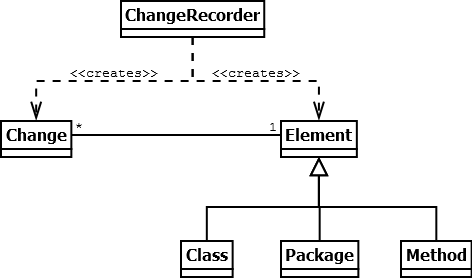
\includegraphics[width=0.8\textwidth]{ChangeLogging}
\caption{Initial design speculation for the change logging functionality}
\label{fig:spec1}
\end{figure}


\section{Reengineering}
text

\section{References}
\begin{thebibliography}{9}

\bibitem{demeyer02}
	Demeyer, Serge, St{\'e}phane Ducasse, and Oscar Nierstrasz,
	\emph{Object-oriented reengineering patterns}. 
	Morgan Kaufmann, 
	2002.

\end{thebibliography}
\end{document}
